\section{Methods}

Using \texttt{Python} in hand with its \texttt{OpenCV} bindings, we created a
program the generates a sequence of images which resemble what a motorist would
likely see while driving through rural, highway, and urban environments. After buffering
the series of images, the program presented the images to a subject. In exactly
half of the images a subject encountered, a cyclist was present with a
different colored tail light. Furthermore, the subject was tasked with finding
a cyclist if one was present, and then to respond in the affirmative if that
was the case. The program records the subjects response as well as the time it
took them to do so.

\smallskip
The images with cyclists in them are synthetic and are constructed in 
a two part process as follows. An example can be seen in Figure \ref{fig:scene}.

\begin{enumerate}

    \item We took two photographs of cyclists found online and using
        \texttt{Adobe Photoshop and Illustrator} we manually cropped out
        everything except the cyclist itself, and then decreased the $\alpha-$
        value making the cyclist look slightly transparent. This was done to
        ensure better blending in the final result. We chose two photographs
        where one cyclist was wearing very bright clothing and one where a
        cyclist was wearing darker clothing. Since we were primarily concerned
        with the affect of the tail light color, we wanted to make sure the
        data reflects any effects of the clothing color on response time as
        well.  For each of the two cyclists images, we created $8$ copies and
        drew a fully visible (max $\alpha-$ value) ``blob'' of a different
        color in the approximate location of where a tail light for a cyclist
        would likely be situated - one copy is left unmodified as a control.
        Therefore, in total there were $16$ unique cyclist images. 

    \item The program reads in each of the $16$ cyclist images, and places it
        within an image still from dash-cam footage captured at night.  The
        location at which the cyclist is placed is chosen at random, but
        constrained to be within the inner $75\%$ of the background image. The
        stills are hand selected from the footage and are chosen in an attempt
        to capture a myriad of lighting conditions, clutter, and perspective.

\end{enumerate}

\vspace{2mm}
\begin{figure}[h!]
    \label{fig:scene}
    \centering$
    \begin{array}{cc}
        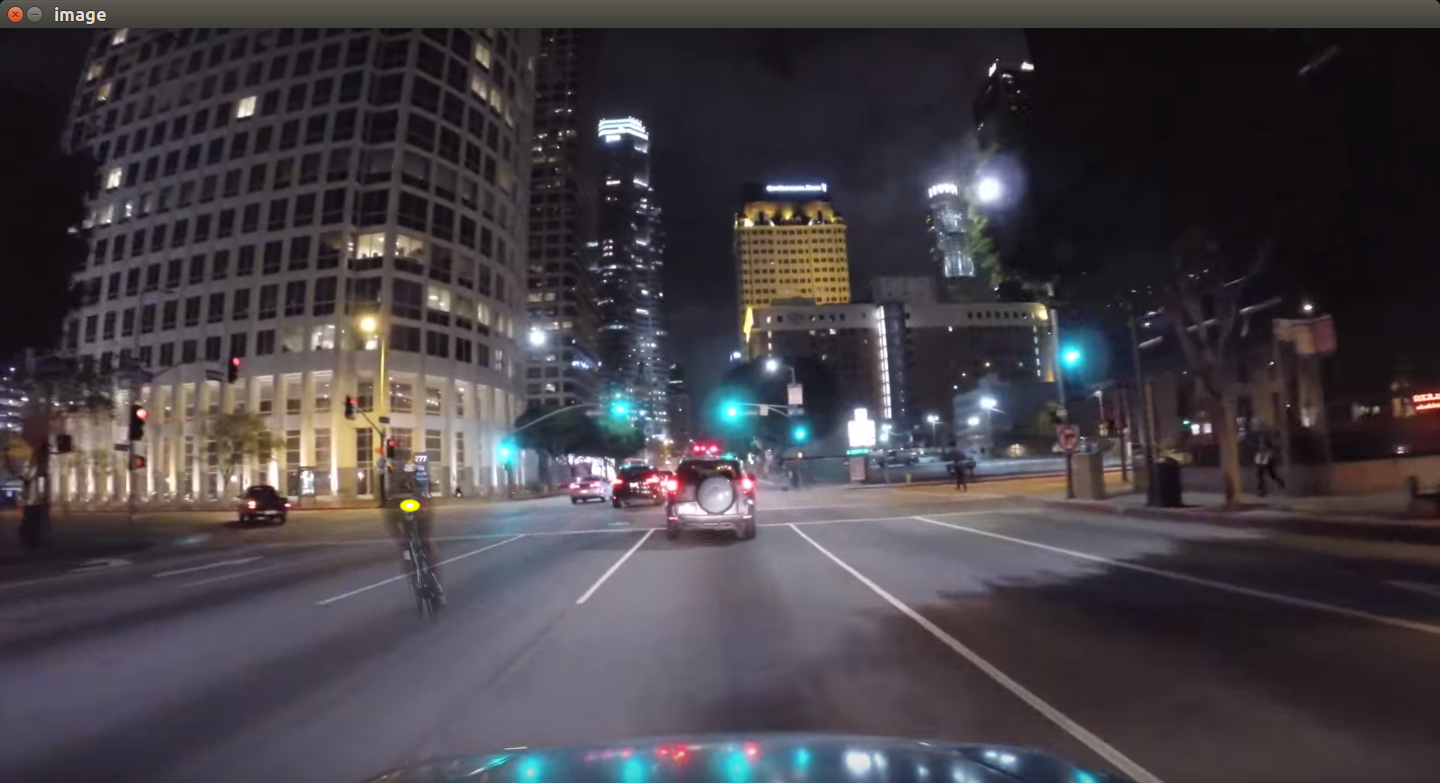
\includegraphics[width=0.8\textwidth]{figures/yellow1.png} \\
        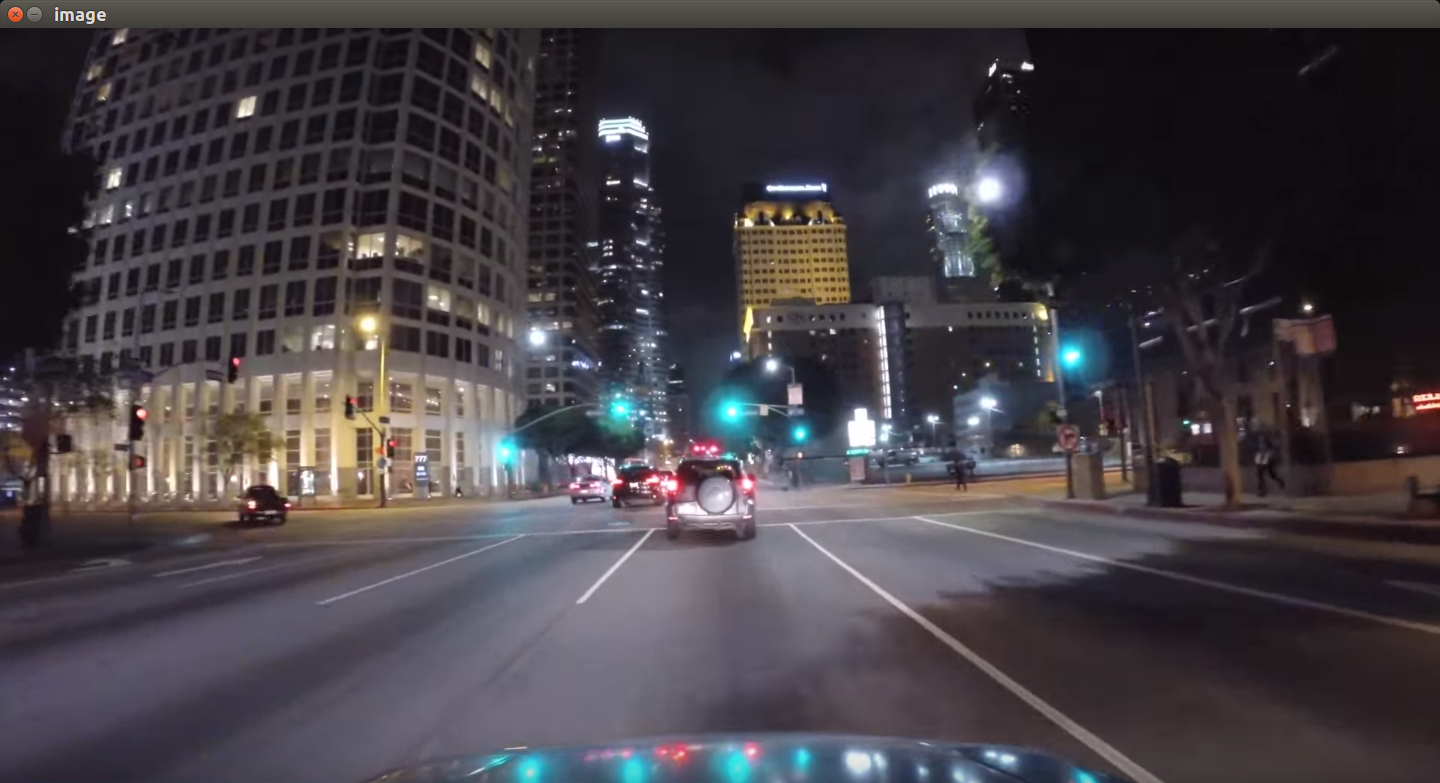
\includegraphics[width=0.8\textwidth]{figures/city1.png}
    \end{array}$
    \caption{ A dash-cam still with and without the embedded cyclist. }
\end{figure}


